\documentclass[a4paper ,12pt, onecolumn]{article}
\usepackage[utf8]{inputenc}
\usepackage[spanish]{babel}

\usepackage[hidelinks]{hyperref}
\usepackage{graphicx}
\graphicspath{ {./images/} }


\begin{document}

\title{Sistemas de posicionamiento de objetos mediante tecnología Bluetooth Low Energy
Beacon }
\author{Rubén Arce}
\date{\today}
\maketitle
\cleardoublepage
\tableofcontents
\cleardoublepage
\section{Memoria descriptiva}
Antecedentes, objeto, normativa, reglamentación
Extensión máxima de 30 páginas + anexos 60
Defensa de 20 min  40
    \subsection{Antecedentes y objeto del proyecto}
    Este proyecto surge como una necesidad de un cliente para llevar a cabo la automatización del puertas
    de su supermercado. 
    \subsection{Ambito de aplicación}
    \subsection{Análisis de soluciones}
    \subsection{Resultados finales}
    \subsection{Planificación}
        \paragraph{}
        Para sintetizar el proceso de desarrollo del proyecto técnico se empleará un diagrama GANTT: 
        \paragraph{}
        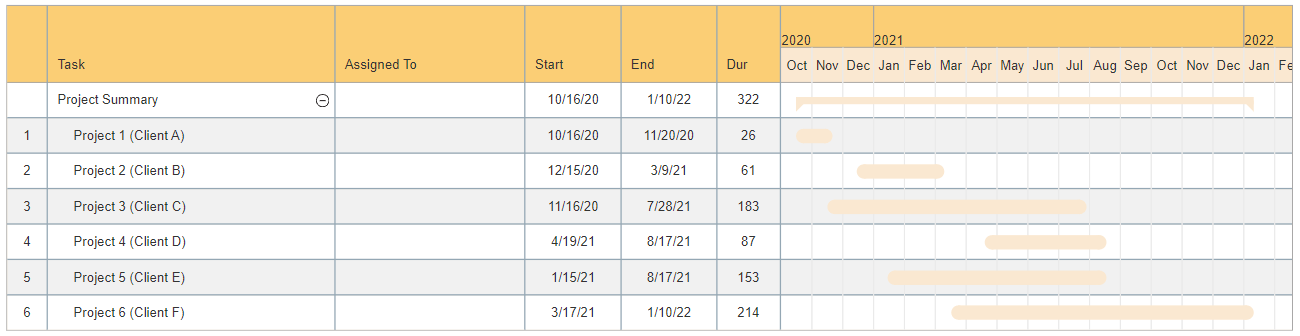
\includegraphics[width=15cm, height=8cm]{gantt.PNG}
        Fase 1: Analisis de la problemática y búsqueda de soluciones
        Fase 2: Prototipos y programación
        Fase 3: Pruebas de campo
        Fase 4: Evolución del equipo en instalación y depuración 
\section{Memoria justificativa}
    \subsection{Calculos justificactivos de la instalación}
        Calculos de consumos de los equipos y dimensionamiento de la batería.
        Los datos de partida son el consumo medio y duración del batería durante 2 años.
\section{Planos}
    \subsection{Plano de mecánicos}
    \subsection{Plano de eléctricos}
        \subsubsection{Esquemático del emisor beacon}
        \subsubsection{PCB circuito del emisor beacon}
        \subsubsection{Esquemático del receptor ESP32}
        \subsubsection{PCB circuito del receptor ESP32}
\section{Pliego de condiciones}
    \subsection{Prescripciones ténicas generales}
        \subsubsection{Normativa relativa a radiofrecuencia}
        \subsubsection{Normativa relativa a }
    \subsection{Prescripciones ténicas particulares}
        \subsubsection{Condiciones que ha de reunir el material}
        \subsubsection{Ejecución del proyecto}
        Placa ha de cumplir solo 1 capa
\section{Presupuestos}
    \subsection{Precios unitarios}
        \begin{center}
            \begin{tabular}{||c | c ||} 
            \hline
            ESP32 Mode & Power consumption  \\ [0.5ex] 
            \hline\hline
            Wi-Fi Tx packet 13dBm~21dBm & 160~260mA  \\ 
            \hline
            \end{tabular}
        \end{center}
    \subsection{Presupuestos Parciales}
        \subsubsection{Capitulo 1: Placa de circuito impreso emisor}
        \subsubsection{Capitulo 2: Placa de circuito impreso receptor}
        \subsubsection{Capitulo 1: }
        \subsubsection{Capitulo 1: }
    \subsection{Presupuestos Total}
        con iva
    \subsection{Factores económicos y financieros}
    Estudio de viabilidad económica
        \subsubsection{Tasa de interés de retorno(TIR)}
        \subsubsection{Valor Actual Neto (VAN)}

\section{Estudio de compativilidad electromagnética}
\subsection{test}
\subsubsection{test}

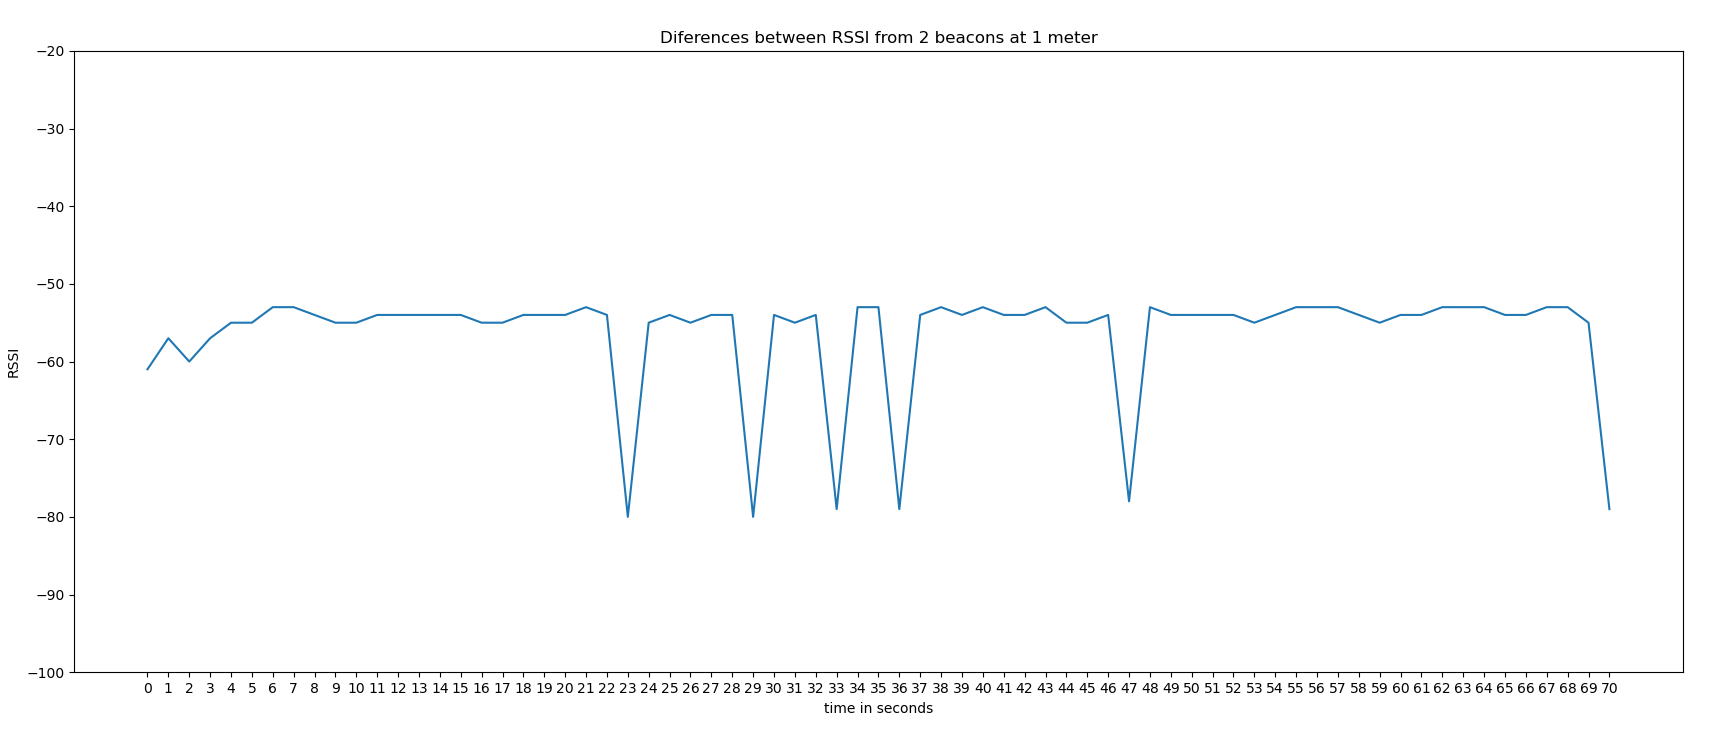
\includegraphics[scale=0.3]{5min_beacon_rssi}
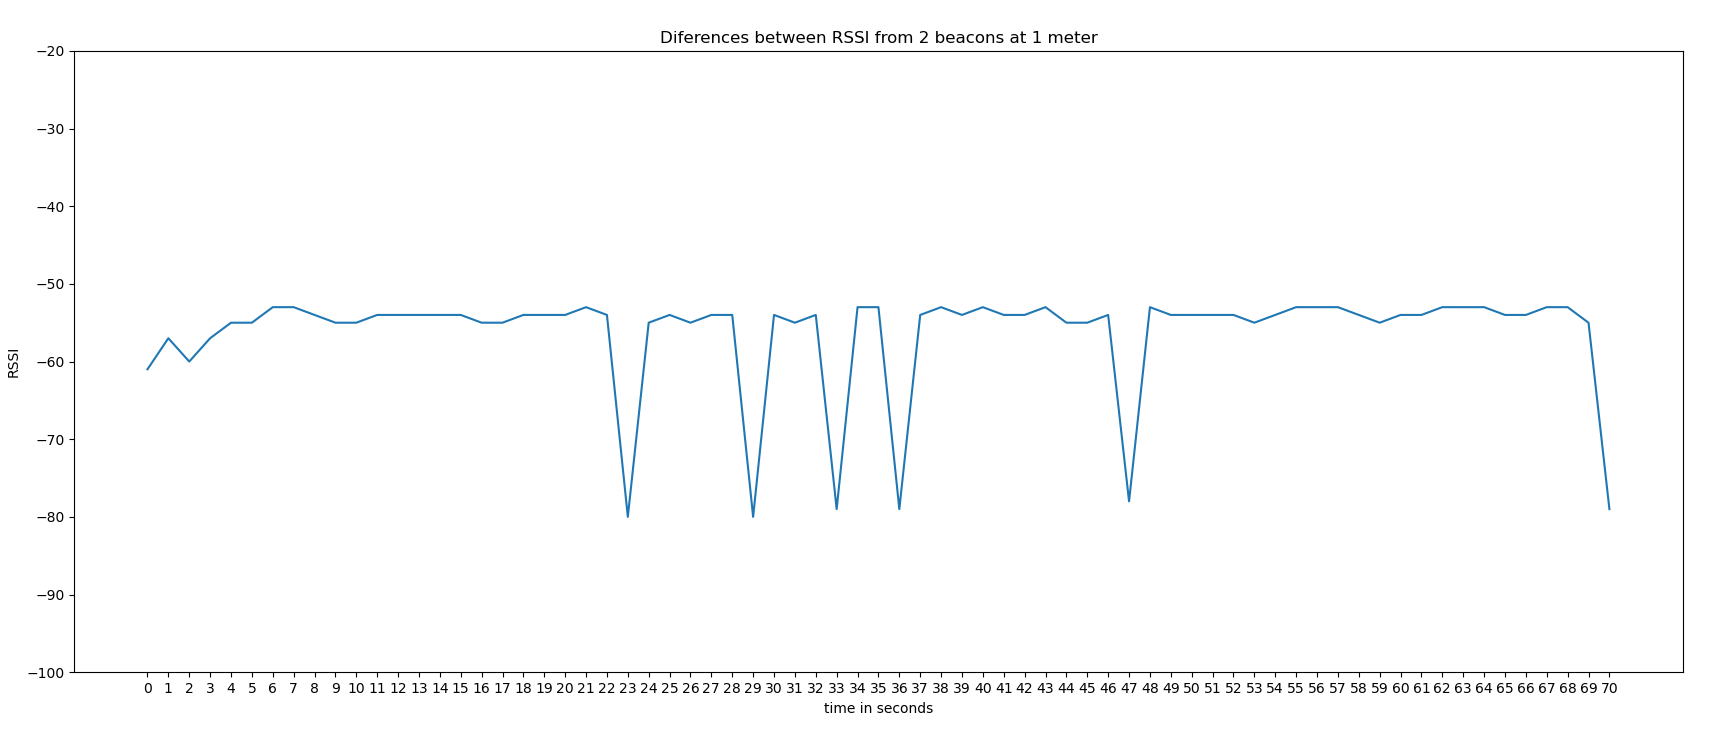
\includegraphics[width=15cm, height=8cm]{5min_beacon_rssi}
\paragraph{hola}
asdfasd


\section{Estado de mediciones}

\section{Bibliografía}
\href{https://campus.masterd.es/campusvirtual/index.htm}{Something Linky} 
\begin{itemize}
    \item  Active mode: 160-260mA.  Active core, ULP coprocessor and RTC
     Wifi, Bluetooth, Radio, Peripherals
    \begin{center}
        \begin{tabular}{||c | c ||} 
        \hline
        ESP32 Mode & Power consumption  \\ [0.5ex] 
        \hline\hline
        Wi-Fi Tx packet 13dBm~21dBm & 160~260mA  \\ 
        \hline
        Wi-Fi/BT Tx packet 0dBm	 & 120mA  \\
        \hline
        Wi-Fi/BT Rx and listening & 80~90mA  \\
        \hline
       \end{tabular}
       \end{center}
    \item  Sleep mode: 3-20mA Active core, ULP coprocessor and RTC
    Inactive: Wifi, Bluetooth, Radio, Peripherals
    \item  Light sleep mode: the CPU is paused by powering off its clock 
    pulses, while RTC and ULP-coprocessor are kept active. This results in 
    less power consumption than in modem sleep mode which is around 0.8mA.

    \item Deep sleep mode, the CPU, most of the RAM and all the digital 
    peripherals are powered off. The only parts of the chip that remains 
    powered on are: RTC controller, RTC peripherals (including ULP 
    co-processor), and RTC memories (slow and fast).
    The chip consumes around 0.15 mA(if ULP co-processor is powered on) to 10µA.

    In Deep sleep mode, power is shut off to the entire chip except RTC module. So, any data that is not in the RTC recovery memory is lost, and the chip will thus restart with a reset. This means program execution starts from the beginning once again.

    \item Hibernation mode: Unlike deep sleep mode, in hibernation mode the chip disables internal 8MHz oscillator and ULP-coprocessor as well. The RTC recovery memory is also powered down, meaning there’s no way we can preserve any data during hibernation mode.

    Everything else is shut off except only one RTC timer on the slow clock and some RTC GPIOs are active. They are responsible for waking up the chip from the hibernation mode.
    
    This reduces power consumption even further. The chip consumes around 2.5µA only in hibernation mode.

    \begin{center}
        \begin{tabular}{||c | c ||} 
        \hline
        ESP32 Mode & Power consumption  \\ [0.5ex] 
        \hline\hline
        Wi-Fi Tx packet 13dBm~21dBm & 160~260mA  \\ 
        \hline
        Wi-Fi/BT Tx packet 0dBm	 & 120mA  \\
        \hline
        Wi-Fi/BT Rx and listening & 80~90mA  \\
        \hline
       \end{tabular}
       \end{center}
\end{itemize}
\begin{enumerate}
    \item  yas
\end{enumerate}
\end{document}